  %%%%%%%%%%%%%%%%%%%%%%%%%%%%%%%%%%%%%%%%%%%%%%%%%%%%%%%%%%%%%%%%%%%%%%
% LaTeX Example: Project Report

%%% Preamble
\documentclass[paper=a4, fontsize=11pt, abstract=on]{scrartcl}
\usepackage[T1]{fontenc}
\usepackage{fourier}
\usepackage{tabularx}
\usepackage[utf8]{inputenc}
\usepackage{hyperref}





\usepackage{listings}
\usepackage{color}

\definecolor{dkgreen}{rgb}{0,0.6,0}
\definecolor{gray}{rgb}{0.5,0.5,0.5}
\definecolor{mauve}{rgb}{0.58,0,0.82}
\lstset{frame=tb,
  language=[Visual]C++,
  aboveskip=3mm,
  belowskip=3mm,
  showstringspaces=false,
  columns=flexible,
  basicstyle={\small\ttfamily},
  numbers=none,
  numberstyle=\tiny\color{gray},
  keywordstyle=\color{blue},
  commentstyle=\color{dkgreen},
  stringstyle=\color{mauve},
  breaklines=true,
  breakatwhitespace=true,
  tabsize=3
}
\usepackage{graphicx}
\usepackage{caption}
\usepackage{subcaption}

\usepackage[english]{babel}															% English language/hyphenation
\usepackage[protrusion=true,expansion=true]{microtype}	
\usepackage{amsmath,amsfonts,amsthm} % Math packages

\usepackage{url}
%\usepackage[hang, small,labelfont=bf,up,textfont=it,up]{caption}


%%% Custom sectioning
\usepackage{sectsty}
\allsectionsfont{\normalfont\scshape}
\usepackage{float}
\usepackage{amsmath}
\usepackage{mathtools}
\usepackage{ragged2e}

\usepackage{nomencl}
\makenomenclature

%%% Custom headers/footers (fancyhdr package)
\usepackage{fancyhdr}
\pagestyle{fancyplain}
\fancyhead{}											% No page header
\fancyfoot[L]{}											% Empty 
\fancyfoot[C]{}											% Empty
\fancyfoot[R]{\thepage}									% Pagenumbering
\renewcommand{\headrulewidth}{0pt}			% Remove header underlines
\renewcommand{\footrulewidth}{0pt}				% Remove footer underlines
\setlength{\headheight}{13.6pt}
   \renewcommand*\abstractname{Summary}

%%% Equation and float numbering
\numberwithin{equation}{section}		% Equationnumbering: section.eq#
\numberwithin{figure}{section}			% Figurenumbering: section.fig#
\numberwithin{table}{section}				% Tablenumbering: section.tab#


%%% Maketitle metadata

\newcommand{\horrule}[1]{\rule{\linewidth}{#1}} 	% Horizontal rule

\title{
		%\vspace{-1in} 	
		\usefont{OT1}{bch}{b}{n}
		\normalfont \normalsize \textsc{} \\ [25pt]
		
\includegraphics[width=0.3\linewidth]{ubc.png} \\
		%
\includegraphics[width=0.4\linewidth]{tru}		
		\horrule{0.5pt} \\[0.2cm]
		\huge Lab \#2 : Measurement of Pressure Distribution, Lift and Drag for an Airfoil \\
		\horrule{2pt} \\[0.005cm]
}
\author{
		\normalfont 								\normalsize
        Jerin Roberts\\[-5pt]		\normalsize
        \today
}
\date{}




%%% Begin document
\begin{document}
\maketitle
\begin{center}
\begin{tabular}{l r}


Supervisor: & Dr. Patrick Kirchen  \\ % supervisor
Locations: & University of British Columbia


\end{tabular}
\end{center}
\newpage
\begin{abstract}
 In this experiment the a Joukowski airfoil will be characterized and its stall angle of attack determined. The drag coefficient, lift coefficient and pressure coefficient were found for varying angles of attack using a wind-tunnel. From this data a approximate stall angle was found for the Joukowski airfoil at 13.5 degrees AOA. Furthermore different methods for calculating the lift coefficient for the airfoil were investigated and found to be in poor agreement with theory and could be further improved with error mitigation or with an improved method of calibration. It was discovered that the airfoil and the plate experience the transition from viscous drag to wave drag at similar Reynolds ranges or more specifically the transition from laminar to turbulent flows.
\end{abstract}


\newpage
\tableofcontents
\listoffigures
\listoftables
\newpage
\lstset{language=[Visual]C++}

\mbox{}% need to run this: makeindex Lab1.nlo -s nomencl.ist -o Lab1.nls

 
\nomenclature{$\rho$}{Density $kg/m^3$}
\nomenclature{$C_D$}{Drag Coefficient}
\nomenclature{$C_L$}{Lift Coefficient}
\nomenclature{$C_P$}{Pressure Coefficient}
\nomenclature{$Re$}{Reynolds Number}
\nomenclature{$A$}{Cross-Sectional Projected Area $m^2$}
\nomenclature{$v$}{Velocity $m/s$}
\nomenclature{$m$}{Mass $kg$}
\nomenclature{$\mu$}{Dynamic Viscosity $Pa-s$}
\nomenclature{$L$}{Characteristic Linear Dimension $m$}
\nomenclature{$q$}{Manometer Reading $mm$}
\nomenclature{$s$}{Airfoil span $m$}
\nomenclature{$c$}{Airfoil chord $m$}
 
\printnomenclature

\newpage
\section{Introduction}

Airfoils are used in many applications and can be found in the fields of transportation, energy production and scientific research. An airfoil is generalized as a body of which contains curved boundaries which are is used to generate lift. The are many properties used to describe the function of an airfoil. Generally lift, drag and pressure profiles for the airfoil will need to be known, as they can be used to help predict how the airfoil will behave. Whether the airfoil is being applied to an aircraft wing or a propeller, the lift, drag and pressure distribution relative to angle of attack will need to be well characterized. In this experiment the a Joukowski airfoil will be characterized and its stall angle of attack determined.

\section{Background}
\subsection{Theory}
\begin{figure}[H]
\centering
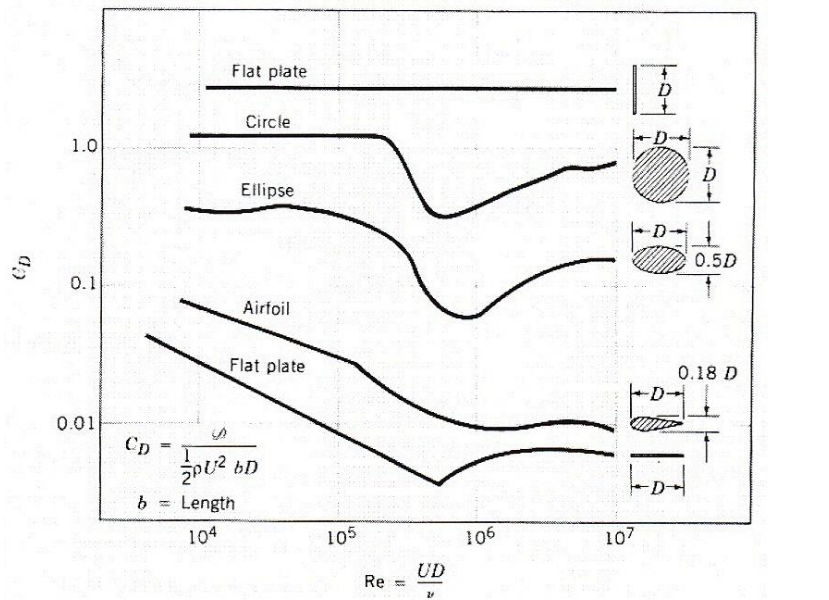
\includegraphics[width=0.8\linewidth]{comp}
\caption{Examples of Drag coefficient as a function of Reynolds number for common objects}
\label{comp}
\end{figure}

For any given airfoil the lift, drag and pressure distribution relative to angle of attack can be characterized. Any object that travels through a fluid will experience an opposing drag force which is related to the objects shape. Drag is generally the result of frictional and viscous forces between the object and fluid. The general expression for force on an object experience due to drag for high Reynolds (above creeping flows) is displayed as equation \ref{drag}.
 \begin{equation}
\label{drag}
F_D= \frac{1}{2}\rho v^2C_DA
\end{equation}

The term $C_D$ is known as the drag coefficient (dimensionless parameter), $F_D$ is the drag force, $\rho$ is the density of the fluid, $v$ is the speed of the object relative to the fluid, and $A$ is the cross sectional area. Similarly Lift is defined as the force on an object perpendicular to the flow direction generated due to its aerodynamic shape. Lift usually results from a pressure imbalance between the top and lower sides of the object causing a net force perpendicular to flow.The pressure difference between the sides is usually generated by the asymmetrical shape of the object. Lift force for high Reynolds flows can be calculated using equation \ref{lift}.

 \begin{equation}
\label{lift}
F_L= \frac{1}{2}\rho v^2C_LA
\end{equation}

The term $C_L$ is known as the lift coefficient, $F_L$ is the drag force, $\rho$ is the density of the fluid, $v$ is the flow speed, and $A$ is the cross sectional area. In this experiment we will investigate these properties for an airfoil and how they are related to angle of attack. 



\section{Methodology}

\subsection{Overview}
Airfoils generally consist of a leading edge, a trailing edge, and a defined by a thickness, camber and cord length. A cross-section of an example airfoil is displayed in figure \ref{fig1}

\begin{figure}[H]
\centering
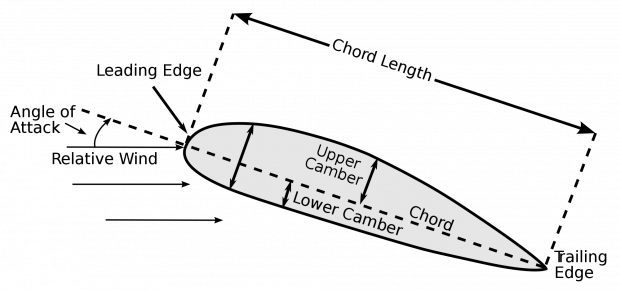
\includegraphics[width=0.8\linewidth]{airfoil}
\caption{A simple diagram of an airfoil cross-section perpendicular to span}
\label{fig1}
\end{figure}
The Joukowski airfoil shape for this experiment is characterized by its chord, span, and thickness. The dimensions for this airfoil are displayed in table \ref{cal}

\begin{table}[H]
\begin{center}
    \begin{tabular}{ | p{0.25\linewidth} | p{0.25\linewidth} |}
 \hline  
     \RaggedRight \textbf{Airfoil Dimension}
    &\RaggedRight \textbf{Specification}
    \\ \hline  
           \RaggedRight chord $c$
    &\RaggedRight 0.3075 m
    \\ \hline 
           \RaggedRight span $s$
    &\RaggedRight 0.6858
    \\ \hline 
           \RaggedRight thickness $h$
    &\RaggedRight 11.1\% $(h/c)$  
    \\ \hline 
    \RaggedRight camber $k$
    &\RaggedRight 2.4\% $k/c)$  
    \\ \hline 
    
    
    \end{tabular}
\end{center} 
\caption{Specifications for Joukowski airfoil}
\label{cal} 
\end{table}

The airfoil is mounted in a wind tunnel to simulate fluid flow over the surface for varying angles of attack. In order to measure the drag and lift forces the airfoil was attached to two load cells, both operate perpendicular to each other for the purpose of measuring lift and drag axis separately. The airfoil is attached to the load cells via a adjustable shaft which allows the angle of attack to be set and measured accurately. Figure \ref{sch} displays a simplified diagram of the experimental setup.


\begin{figure}[H]
\centering
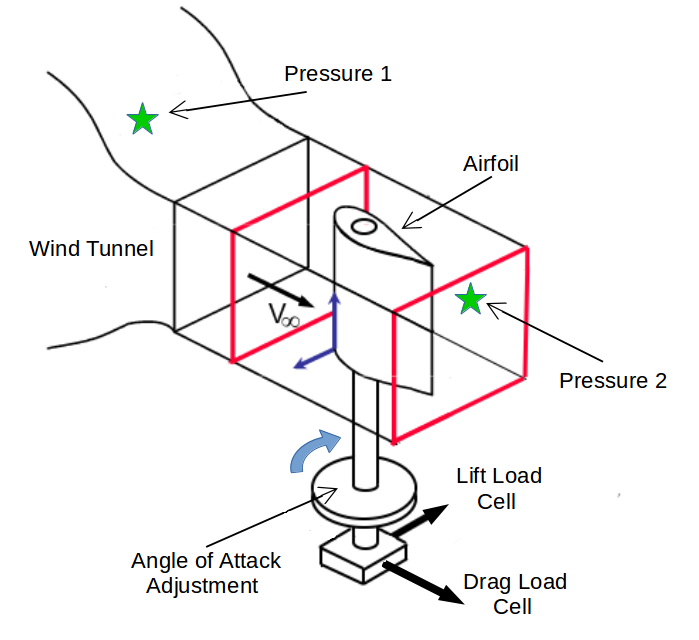
\includegraphics[width=0.8\linewidth]{schem}
\caption{A simple diagram of the experimental setup to measure drag and lift on an airfoil}
\label{sch}
\end{figure}

 Two pressure taps are mounted inside the tunnel, one before and one inside the reduction and are used as references to measure the free flow pressure and the surface pressure on the airfoil. A Betz Manometer is used to calculate the flow velocity. The airfoil has built-in multi-tube manometer which enables discrete pressure measurements on the objects surface. The arrangement of the pressure taps for the airfoil are found in the appendix.

 

\subsection{Calibration}
Calibration was needed to know the relation between measured voltage on load cells vs the forces applied. Subsequent weights in increasing mass were added to a pulley which exerted a force normal to the load cells operating axis. A calibration curve was created for both the drag and lift load cells and is displayed in figure \ref{cal}.

\begin{figure}[H]
\centering
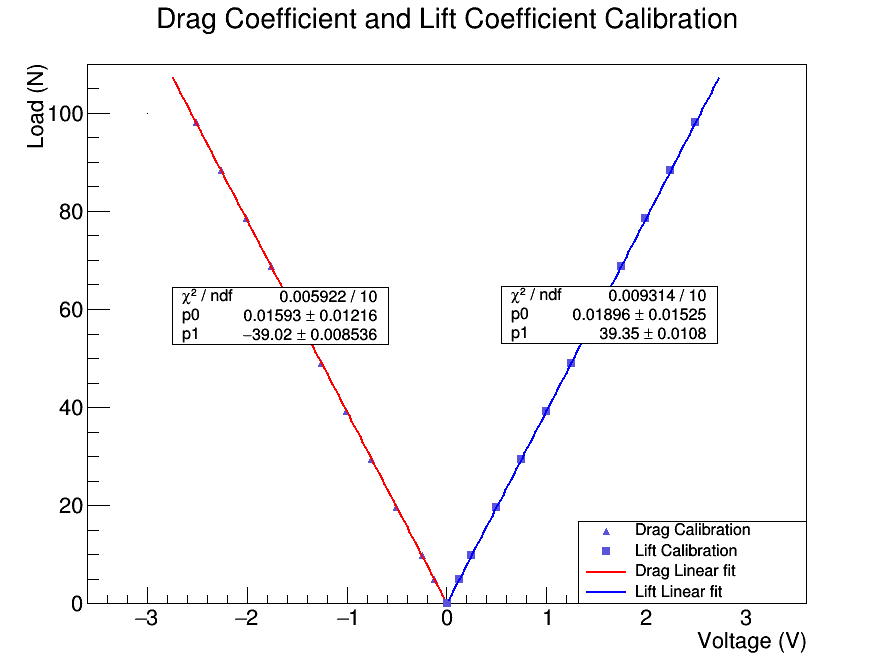
\includegraphics[width=\linewidth]{cali}
\caption{The calibration curve generated to accurately calculate drag and lift forces}
\label{fig1}
\end{figure}

The equations for calculating drag and lift forces are displayed in figure \ref{cal} as 1st order polynomials with the uncertainties for each fitted parameter.

\subsection{Procedure}
For measuring the lift, drag and pressure distribution, the Betz manometer was kept at a constant q = 30 mm of water, while measurements were taken at 2 degree increments from -4 degrees AOA to beyond stall. During each AOA step the  multi-tube manometer pressure distribution was observed qualitatively. When 6 degrees AOA was reached the pressure distribution around the airfoil was recorded using the multi-tube manometer. In order to characterize the drag relative to Reynolds number the airfoil was set at the angle of incidence for minimum lift and drag (ie $\alpha =-4$), and drag was measured at different values of q up to the maximum fan motor speed of 1000 RPM. The data was plotted and analyzed to obtain stall angle for the airfoil.

\subsection{Analysis}
 In our analysis of the drag and lift forces acting on an airfoil for different angles of attack its best to describe the experiment data in a more general way for comparison to other experiments. Lift and Drag coefficients are an effective method of comparing lift and drag effects among objects of different sizes and shapes. The drag coefficient can be calculated using equation \ref{drag}. Rearranging and substituting in for velocity and area we get equation \ref{edrag}
 
 \begin{equation}
\label{edrag}
C_D= \frac{2F_D}{\rho4.03^2 q s c}
\end{equation}

Where $q$ is $mm$ measure on the Betz Manometer, $s$ is the span of the airfoil, $c$ is the chord, $\rho$ is the air density at 20 degrees Celsius and $F_D$ is the force measured by the load cell. Similarly the lift equation was evaluated in the same manner as seen in equation \ref{elift}


 \begin{equation}
\label{elift}
C_L= \frac{2F_L}{\rho4.03^2 q s c}
\end{equation}

The drag and lift forces were calculated for angles of attack ($\alpha$) for a range from -4 to 16 in increments of 2 degrees. The approximate stall angle for the airfoil was then determined. Both the drag and lift coefficient curves were fit with theoretical functions. The drag was fit with a $1/\alpha^2$ while the lift with a 6th order polynomial. Pressure was measured for discrete points on the suction and pressure sides of the airfoil. The multi-tube manometer gives a change in fluid level as a method for measuring pressure difference. Equation \ref{sixy} was used to calculate the pressure at the surface of the airfoil.


\begin{equation}
\label{sixy}
P = (\rho_{fluid}-\rho_{air})g h \sin \theta 
\end{equation}

 Where theta is equal to 60 degrees, $P$ is the pressure difference relative to atmosphere, $g$ is gravity and $h$ is the height displacement of the fluid in the manometer. The pressure surrounding the airfoil was measured using the multi-tube manometer for varying steps of $\alpha$ and is displayed in figure \ref{mult}. For a specific angle of attack the pressure coefficient over the surface can be integrated to calculate the lift coefficient. For integration the trapezoidal rule was used via software to sum the pressure distribution with respect to x which is displayed in equation \ref{trap}. The pressure coefficient can be solved using equation \ref{cp}.
  

\begin{equation}
\label{trap}
C_L = \sum_{i=1}^{35} \frac{C_{P(i)}+C_{P(i+1)}}{2}\triangle x_i
\end{equation}


\begin{equation}
\label{cp}
C_P= \frac{2(P-P_{\infty})}{\rho_{\infty}4.03^2 q}
\end{equation}


\begin{figure}[H]
\centering
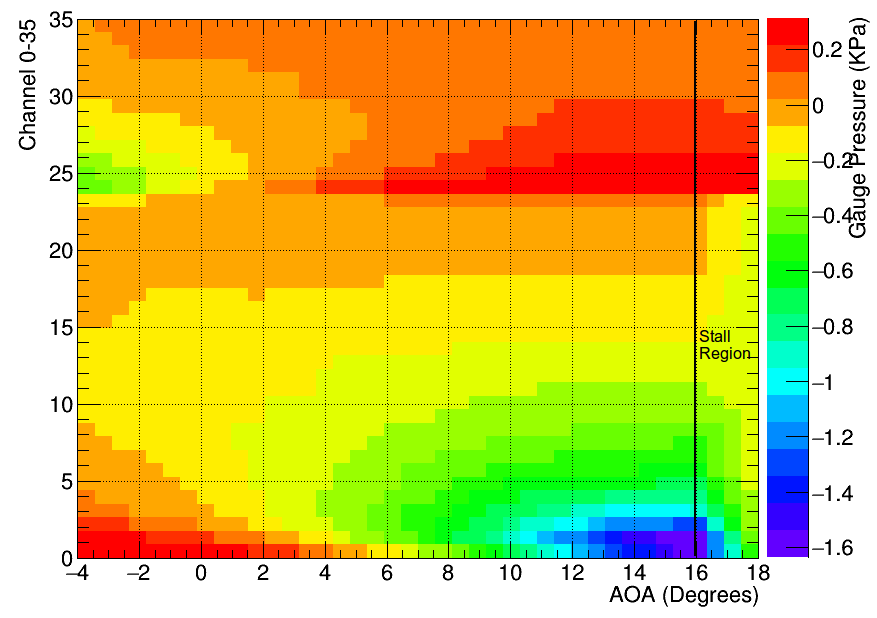
\includegraphics[width=\linewidth]{m1}
\caption{Pressure as a function of channel (y axis) and angle of attack (x axis) at the airfoil surface}
\label{mult}
\end{figure} 
 
\subsection{Uncertainty} 
The uncertainty for the drag and lift measurements was calculated by applying taylor series expansion method to equations \ref{elift} and \ref{edrag}. The resulting application for lift coefficient is displayed in equation \ref{taylor}.


\begin{equation}
\label{taylor}
\delta C_L = C_L \Bigg(\Bigg(\frac{\delta F_L}{F_L}\Bigg)^2+\Bigg(\frac{\delta T}{T}\Bigg)^2+\Bigg(\frac{\delta P_{\infty}}{P_{\infty}}\Bigg)^2+\Bigg(\frac{\delta q}{q}\Bigg)^2\Bigg)^{\frac{1}{2}}
\end{equation}

The uncertainty in the density is a result of the ambient temperature measurement and free-stream pressure measurement, while the error in the velocity is dependent on the error of q from the Betz manometer. Similarly for drag the error was calculated as displayed in equation \ref{tay}

\begin{equation}
\label{tay}
\delta C_D = C_D \Bigg(\Bigg(\frac{\delta F_D}{F_D}\Bigg)^2+\Bigg(\frac{\delta T}{T}\Bigg)^2+\Bigg(\frac{\delta P_{\infty}}{P_{\infty}}\Bigg)^2+\Bigg(\frac{\delta q}{q}\Bigg)^2\Bigg)^{\frac{1}{2}}
\end{equation}
\newpage 
   
\section{Results}

\subsection{Overview}
The results for lift and drag coefficient relative to $\alpha$ are displayed in figure \ref{fig2} The stall angle for the airfoil can be determined by examining the curve for lift coefficient. The point of maximum Cl represents the location of were a may will begin to occur. The maximum Cl for maximum $\alpha$ represents the point at which increasing $\alpha$ will only result in loss of lift which is by definition a stall event. The stall angle for this airfoil was found to be roughly 13.48 degrees $\alpha$ given a fluid velocity of $22m/s$. Note the uncertainty bars for lift and drag coefficient have been scaled up for visualization purposes (5x). It should be noted that the error for $C_D$ and $C_L$ are large for large values of $\alpha$. This is due to the turbulent regions generated while nearing the stall angle. The sharper the angle of attack the more likely separation is to occur. This can cause the airfoil to vibrate introducing large errors in the force measurement.


\begin{figure}[H]
\centering
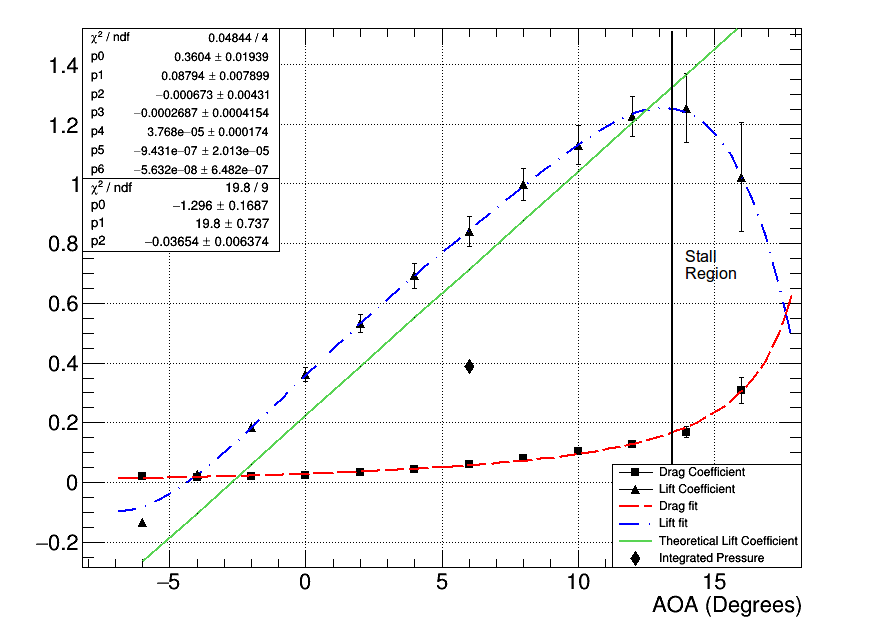
\includegraphics[width=0.8\linewidth]{q1}
\caption{Lift and Drag coefficient relative to $\alpha$ (AOA). Errors are scaled (5x)}
\label{fig2}
\end{figure}

Figure \ref{fig2} shows the results of 3 different methods for calculating lift coefficient. The first is calculated with experimental force measurements, the 2nd with the pressure coefficient for a single $alpha$, and the last is a theoretical model. The 3 methods do not agree well with each other. The theoretical plot and experimental plot both share similar slopes and therefore their large offset difference may be a result of a calibration error. The large difference between the pressure calculated value of $C_L$ and the theoretical may be a result of descretization. Adding more taps may more accurately predict the pressure distribution around the airfoil and therefore provide a more accurate value for $C_L$.





\begin{figure}[H]
\centering
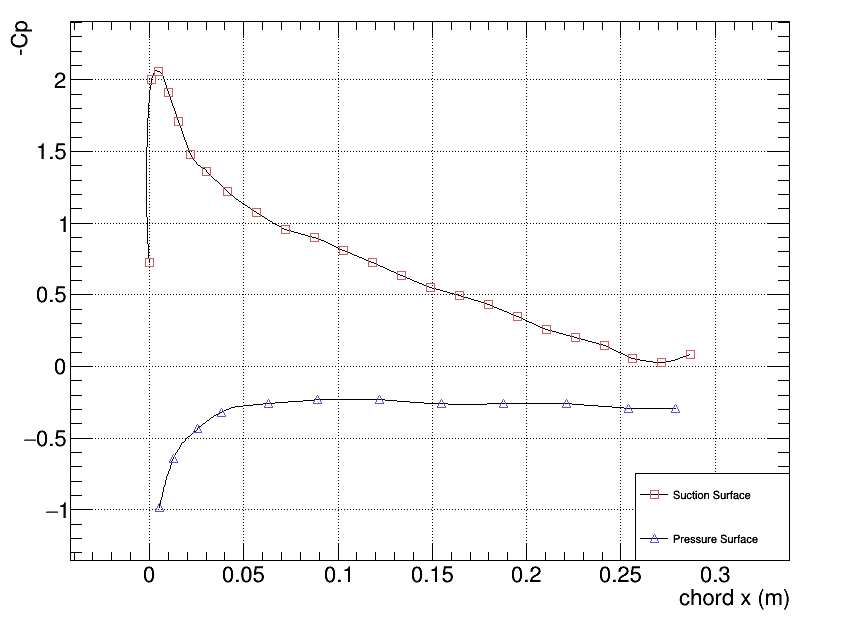
\includegraphics[width=0.7\linewidth]{p1}
\caption{Pressure coefficient vs Chord length c for $\alpha$=6}
\label{press}
\end{figure}

Figure \ref{press} displays the calculated pressure coefficient for discrete points around the airfoil and are plotted relative to chord length. The pressure side has positive values of Cp while the suction side has negative values of Cp. When Cp is equal to zero the pressure is equal to the free-flow pressure, while a Cp of 1 indicates a stagnation point. Note values of Cp cannot be greater than one. The curve in figure \ref{press} when integrated over the surface will result in the lift coefficient. The lift coefficient calculate from pressure distribution around airfoil was found to be 0.388.
Figure \ref{re} displays the drag coefficient measured relative to Reynolds number. 


\begin{figure}[H]
\centering
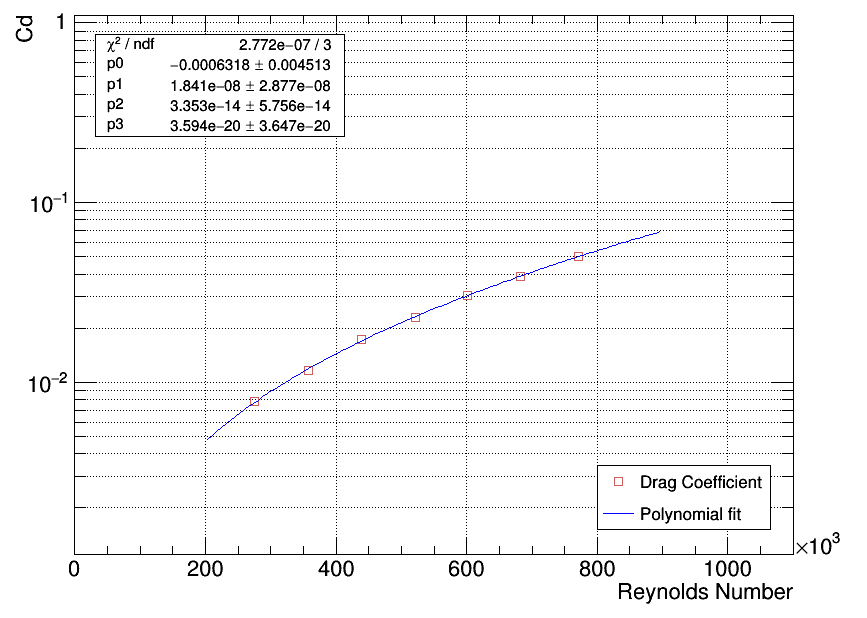
\includegraphics[width=0.7\linewidth]{r1}
\caption{Drag Coefficient vs Reynolds number for Joukowski airfoil}
\label{re}
\end{figure}
This data was compared against the plot in figure \ref{comp} for reference. The general shape and range of the curve agrees relative to the objects in figure \ref{comp} as the Joukowski airfoil lies somewhere between the $C_D$ for a plate and a symmetric elongated teardrop. We could not expect an exact match as the shapes are very different. Its clear though from these plots that the airfoil and the plate experience the transition from viscous drag to wave drag at similar Reynolds ranges or more specifically the transition from laminar to turbulent flows.

\section{Conclusion}
In this experiment we successful characterized the drag and lift coefficient for varying angles of attack. From this data a approximate stall angle was found for the Joukowski airfoil. Furthermore different methods for calculating the lift coefficient for the airfoil were investigated and found to be in poor agreement with theory and could be further improved with error mitigation or with an improved method of calibration. It was discovered that the airfoil and the plate experience the transition from viscous drag to wave drag at similar Reynolds ranges or more specifically the transition from laminar to turbulent flows. This experiment provided a great base for understanding the considerations necessary when making measurements regarding pressure, drag and lift with respect to fluid flow.





\newpage



\appendix
\section{Appendix} \label{App:Appendix}
\subsection{Joukowski Airfoil Pressure Tap}

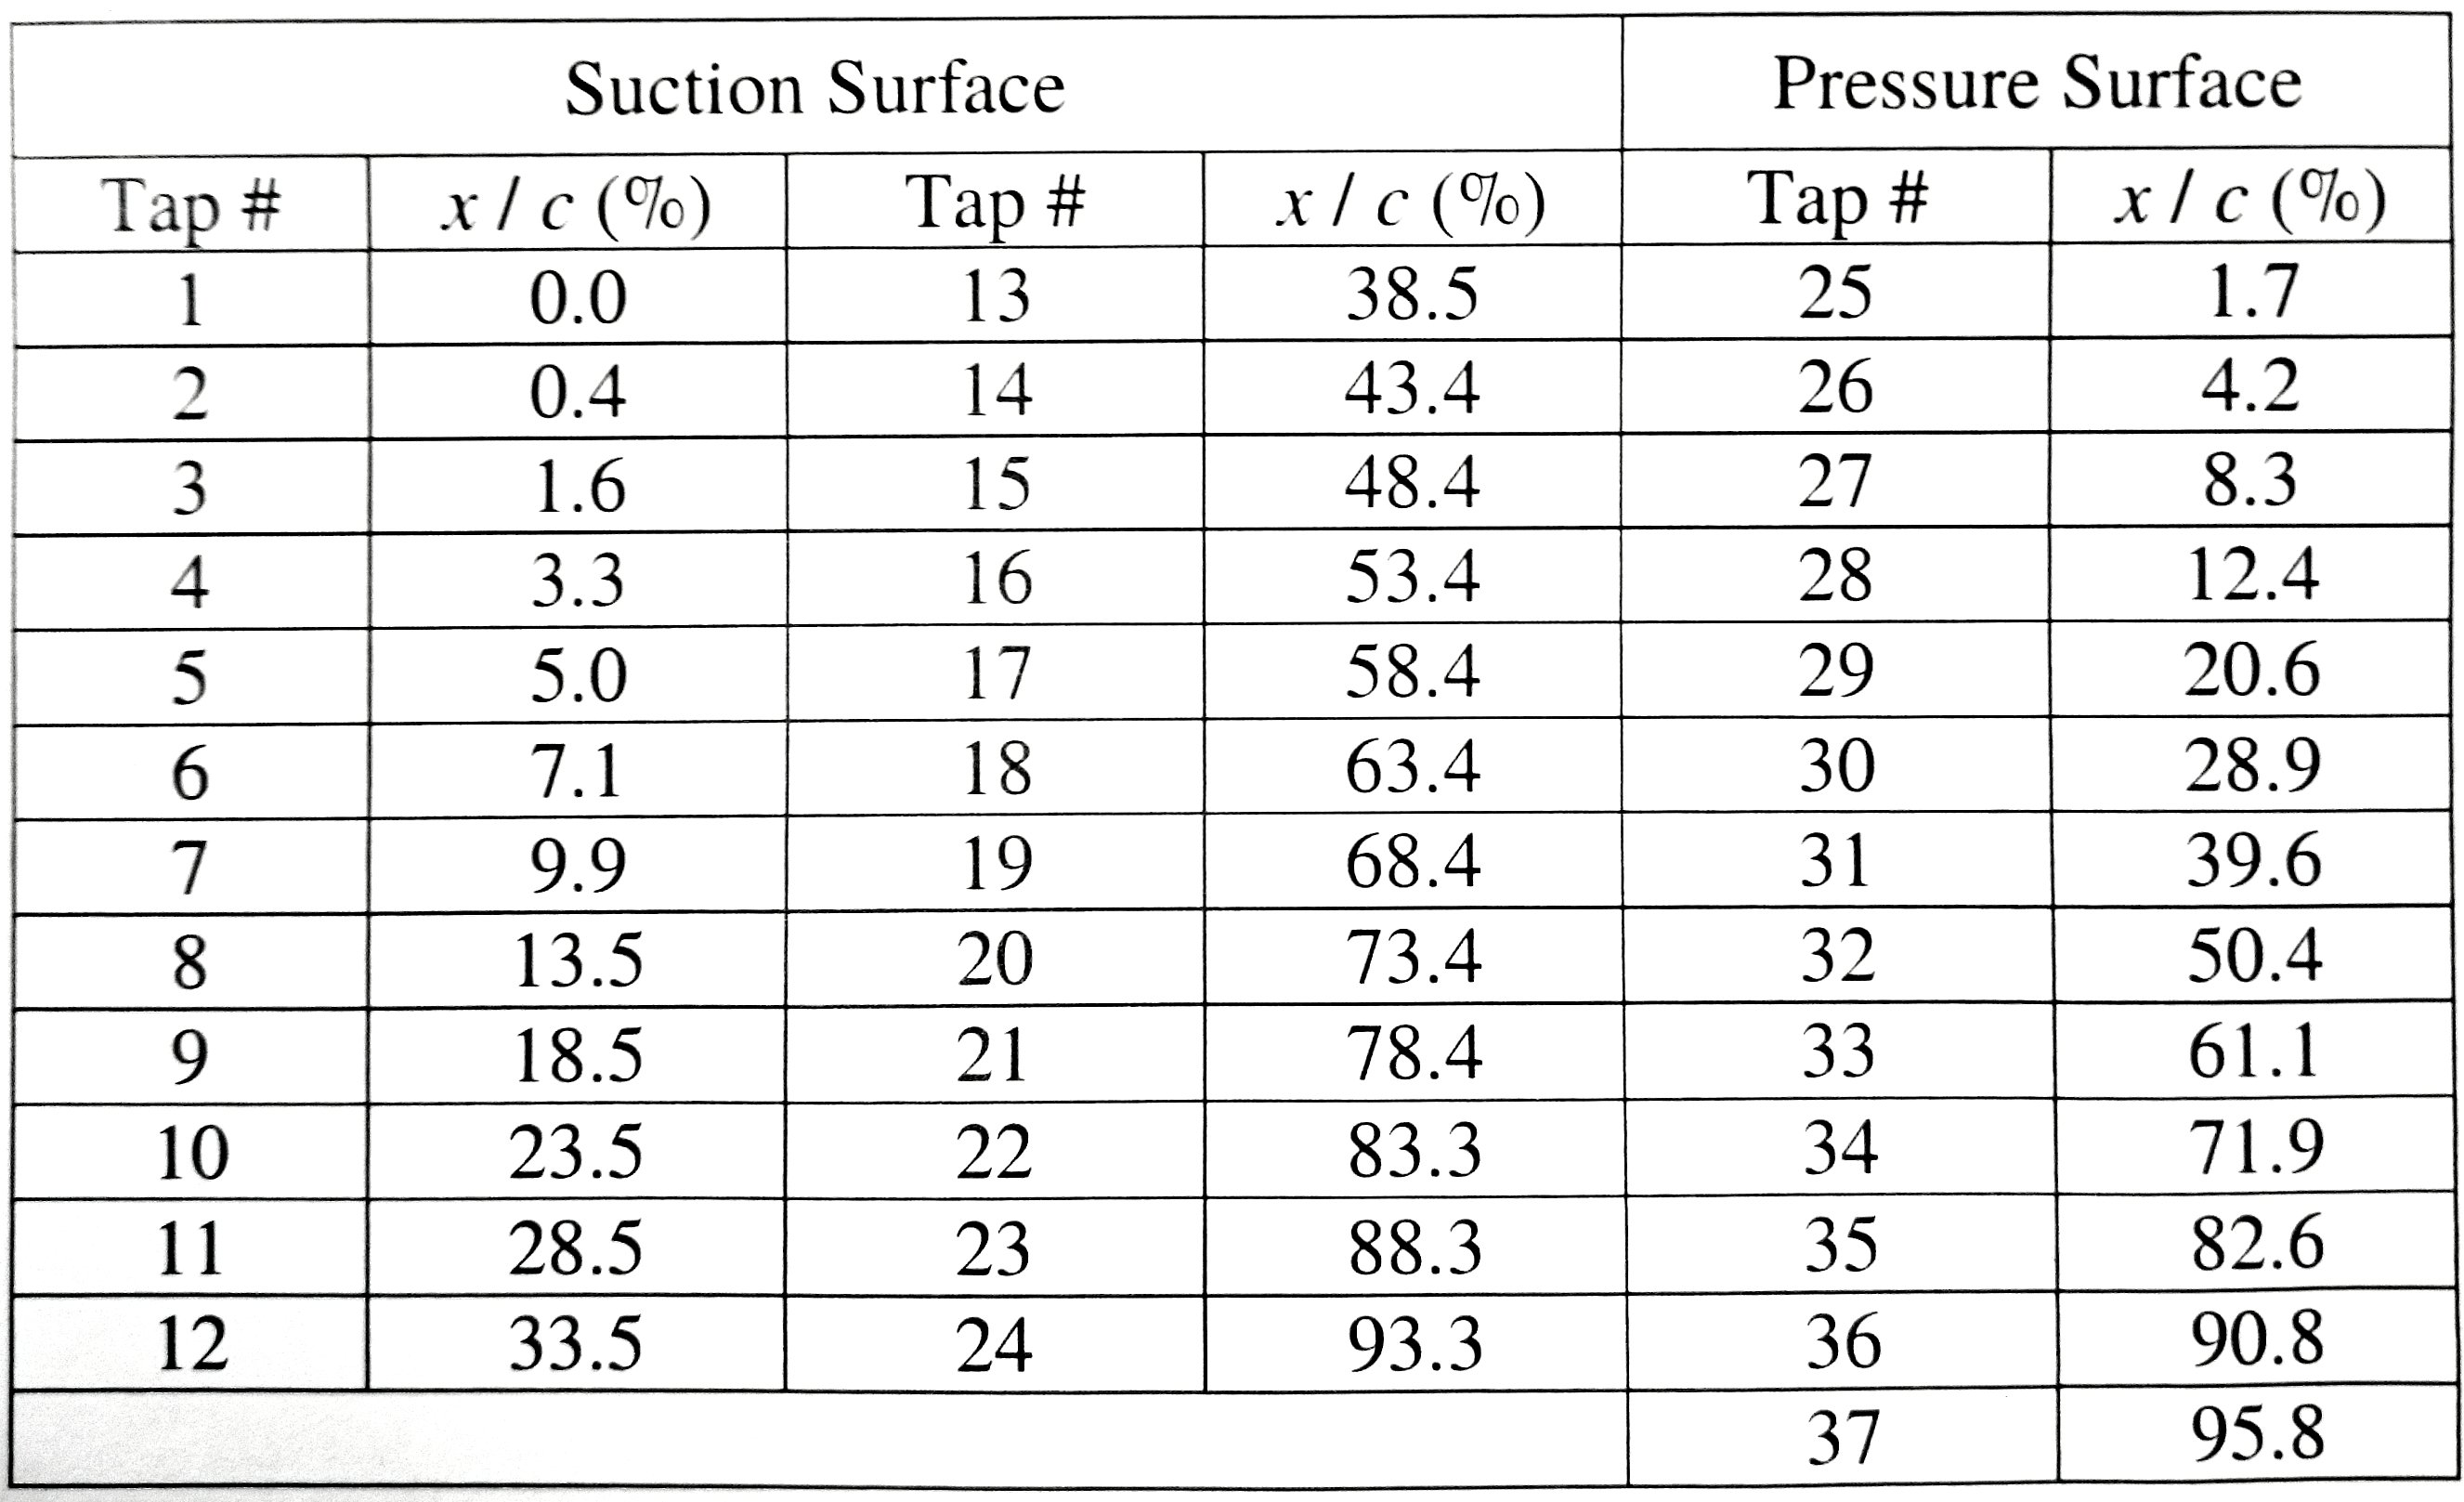
\includegraphics[width=0.8\linewidth]{table}

\subsection{Betz Manometer}


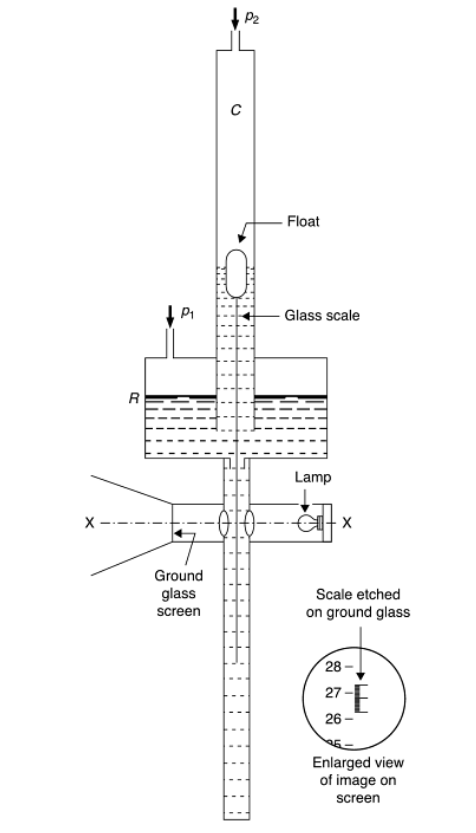
\includegraphics[width=0.8\linewidth]{betz}


\subsection{}




\begin{thebibliography}{99} % Beamer does not support BibTeX so references must be inserted manually as below

\bibitem[Cimbala, 2012]{p2} J.M. Cimbala (1999)
\newblock "Drag on Spheres", Department of Engineering, Penn State Univeristy
\end{thebibliography}


%%% End document
\end{document}